
\section{Implementação do Padrão de Visitante (\texttt{walker})} \label{section-walker}


Desenvolvemos o pacote \texttt{walker} para auxiliar em quatro tarefas-chave: inferência de tipos das expressões, validação da precedência da AST gerada pelo \textit{parser}, visualização gráfica da AST, e geração de código. Para atingir esses objetivos, empregamos o padrão de projeto \textit{visitor} \footnote{\url{https://refactoring.guru/pt-br/design-patterns/visitor}}, que facilita a travessia e manipulação da AST. A estrutura principal do pacote consiste em duas peças fundamentais: a estrutura \texttt{Visitor} e a função \texttt{walk}.

\subsection{Estrutura \texttt{Visitor}}

A estrutura \texttt{Visitor} (\autoref{cod-visitor-struct}) encapsula uma função de visita polimórfica (\texttt{visit}) que pode ser invocada em cada nó da AST. Essa abordagem permite que a lógica de manipulação da AST seja flexível e extensível. A função \texttt{visit} pode ser definida nessa estrutura para realizar operações transformação de nós, como mudar o campo \texttt{ty\_inferred} do nó do tipo \texttt{Expr}; também é permitido remoção ou adicição de nós. Além disso, a estrutura permite que o visitante mantenha um estado interno (\texttt{data}), que pode ser modificado dinamicamente durante a travessia. Como exemplo, esse estado é usado para manter um inteiro indicando a profundidade atual para gerar um SVG da arvóres \autoref{SVG}, ou uma lista de indentificadores usados para fazer resolução de simbolos pelo pacote \texttt{checker}, entre outros usos.

% A estrutura \texttt{Visitor} (\autoref{cod-visitor-struct}) encapsula uma função de visita polimórfica que pode ser chamada para cada tipo de nó, possibilitando um processamento flexível e extensível, onde o visitante pode modificar seu próprio estado durante a travessia, decidir continuar ou interromper o caminhamento, e realizar operações arbitrárias como transformação, análise semântica, geração de código ou depuração.


\subsection{Função \texttt{walk}}
A função \texttt{walk} (\autoref{cod-visitor-walk}) implementa um mecanismo genérico e recursivo de travessia profunda (\textit{depth-first}) da AST. Essa função percorre todos os nós, incluindo declarações, expressões e equações e definição de funções, aplicando a função \texttt{visit} antes e depois de explorar cada subárvore. Isso é especialmente útil para criar \textit{visitors} personalizados para tarefas como:

\begin{itemize}
    \item Checagem de tipos: Verifica a consistência dos tipos em diferentes nós da árvore.
    \item Parentização de expressões: Modifica nós para assegurar precedência correta de operadores.
    \item Geração de gráficos: Produz uma representação visual em arquivo no formato SVG da AST.
    \item Geração de código: Traduz a AST para uma linguagem GLSL.
\end{itemize}

O controle de parada em \texttt{walk} é essencial para evitar chamadas recursivas desnecessárias ou operações em nós inválidos. Este controle é realizado por meio de duas verificações principais

Verificação de nulidade: A função verifica se o visitante (\texttt{v}) ou o nó (\texttt{node}) atual são nulos antes de proceder. Isso garante que a execução não tente operar em dados inexistentes.

Interrupção de travessia: Após cada chamada à função \texttt{visit}, verifica-se o retorno do visitante. Se for \texttt{nil}, a travessia é interrompida, permitindo que o \textit{visitor} decida dinamicamente se deseja continuar ou parar; adaptando-se a diferentes cenários de análise e manipulação da AST.



\begin{codigo}[!ht]
    \caption{\small Estrutura polimórfica \texttt{Visitor}}
        \label{cod-visitor-struct}
\begin{lstlisting}[language = C]

// Estrutura polimórfica, aceita um tipo qualquer, chamado de DataType, como estrada para criar um tipo concreto.
Visitor :: struct (DataType: typeid) {
    visit: proc(visitor: ^Visitor(DataType), node: ^ast.Node) -> ^Visitor(DataType),
    data:  DataType,
}
\end{lstlisting}
\end{codigo}

\begin{codigo}[!ht]
\caption{\small Função de percurso \texttt{walk}. }
        \label{cod-visitor-walk}
\begin{lstlisting}[language = C]
// Por brevidade vamos omitir varios casos do `switch` que seguem a mesma lógica
walk :: proc(v: ^Visitor($T), node: ^ast.Node) {
    if v == nil || node == nil {
        return
    }
    v := v->visit(node)
    if v == nil {
        return
    }
    using ast
    switch n in &node.derived {
        case ^Start:
            for d in n.decls {
                walk(v, d)
            }

        case ^Decl_Equation:
            walk(v, n.field)

        case ^Field:
            walk(v, n.name)
            walk(v, n.value)

        case ^Expr_Number:     // Caso base

        case ^Expr_Vector_Literal:
            for number in n.numbers {
                walk(v, number)
            }
        case ^Expr_Identifier:
                walk(v, n.sub_expression)

        // ...
        // casos OMITIDOS aqui Também
        // ...
        case ^Expr_Infix:
            walk(v, n.left)
            walk(v, n.right)

        case ^Expr_Grouped:
            walk(v, n.expr)

        case ^Expr_Function_Call:
            walk(v, n.left)
            for e in n.exprs {
                walk(v,  e)
            }
        case:
            assert(false, "Unhandled token on walk_print ")
    }
    v = v->visit(nil)
}

  \end{lstlisting}
\end{codigo}


\subsection{Validação de Precedencia}

Utilizamos o pacote \texttt{walker} para validar a precedência dos operadores na AST gerada pelo \texttt{parser}. A função de parentização implementa a inserção de parênteses para capturar a precedência original das expressões da AST. Dessa forma, a representação textual resultante reflete corretamente a ordem de avaliação das expressões matemáticas.

Durante a travessia da AST, o algoritmo processa todos os tipos de expressões, como prefixas, binárias e chamadas de função, inserindo parênteses sempre que necessário. Isso garante que a hierarquia das operações seja explicitamente representada, permitindo verificar se a construção da AST durante o parsing respeitou corretamente as regras de precedência matemáticas.

Os testes de precedência consistem em comparar o texto original de uma expressão com sua versão esperada, na qual os parênteses refletem a ordem de avaliação correta (\autoref{cod-test-paren}). Casos mais complexos, como a combinação de operadores associativos à direita (como a exponenciação) com operadores de diferentes precedências, são incluídos para abranger cenários que envolvem todas as operações aritméticas suportadas. Além disso, as expressões podem conter sub-expressões aninhadas, chamadas de funções e expressões como parâmetros na definição de funções.

À medida que o compilador foi sendo desenvolvido, esses testes se mostraram úteis para evitar regressões. Sempre que uma nova funcionalidade era adicionada, os testes garantiam que funcionalidades já existentes não fossem quebradas.


%%%%


\begin{codigo}[htb]
    \caption{\small Validação de precendencia por parentização de expressões. }
        \label{cod-test-paren}
  \begin{lstlisting}[language = C]
    test_paren(
        "a = 1+2", // Entrada
        "a=(1+2)"  // Saída Esperada
    );

    test_paren(
        "a = \exp 1 + 2^3", // Entrada
        "a=(\exp(1)+(2^3))" // Saída Esperada
    );

    // ...
    // Outros Testes
    // ...

    test_paren(
        "a = a(1*2 ^ 4 +  \sqrt 4^8 , 2)", // Entrada
        "a=a(((1*(2^4))+(\sqrt(4)^8)),2)"  // Saída Esperada
    );
  \end{lstlisting}
\end{codigo}



\subsection{Visualização da AST por Imagem}

Para validação visual, foi implementado uma função que gera uma imagem da AST no formato SVG, que é textual e fácil de manipular. Cada nó da AST é representado por um retangulo com textos associados que fornecem informações, como o tipo de operador, o tipo do nó e a string do identificador, se aplicavel. Anteriormente, utilizávamos a função \texttt{print\_ast}, que imprimia os nós e seus atributos com indentação correspondente à profundidade. Essa abordagem se tornou limitada à medida que a AST crescia em complexidade, demandando uma solução mais robusta para depuração.

Na \autoref{fig-svg}, apresentamos a visualização gerada para a equação \autoref{eq-svg}. Observamos que os nós de operações binárias, como \texttt{+} e \texttt{-}, localizados próximos à raiz, são avaliados posteriormente, enquanto os nós mais próximos das folhas, como \texttt{*} e \texttt{\^}, têm maior precedência e são resolvidos primeiro. Além disso, o SVG inclui informações adicionais, como o tipo das expressões. Por exemplo, o identificador \( f \) é anotado como pertencente ao tipo \( \mathbb{R} \), o que é determinado na etapa de validação semântica (\texttt{checker}), como será discutido posteriormente.

Os nós da AST são heterogêneos, e o modo de acessar seus filhos varia conforme o tipo do nó, já que os campos podem ter nomes ou posições diferentes nas estruturas. Para lidar com essa heterogeneidade, o pacote \texttt{walker} oferece uma função chamada \texttt{children} (\autoref{cod-childre-signature}). Essa função abstrai as diferenças entre os tipos de nós e retorna, para qualquer nó, uma lista uniforme de seus filhos. Isso simplifica o código de geração do SVG, permitindo que a função opere sobre a AST de maneira uniforme, sem a necessidade de tratar cada tipo de nó individualmente.
%%%%%%%
\begin{equation} \label{eq-svg}
   f =  1*2 ^ 4 +  \sqrt 4^8
\end{equation}


\begin{codigo}[!h]
        \caption{\small Assinatura da função que extrai nós filhos de maniera uniforme para qualquer tipo de nó. }
        \label{cod-childre-signature}
  \begin{lstlisting}[language = C]
    // Aceita um ponteiro de nós abstrato e return uma lista de nós filhos
    children :: proc(node: ^Node) -> (array :[dynamic]^Node);
  \end{lstlisting}
\end{codigo}

% \begin{figure}[H]
\begin{figure}[!h]
    \caption{\label{fig-svg} \small SVG da AST gerado para \autoref{eq-svg}.}
    \begin{center}
        % 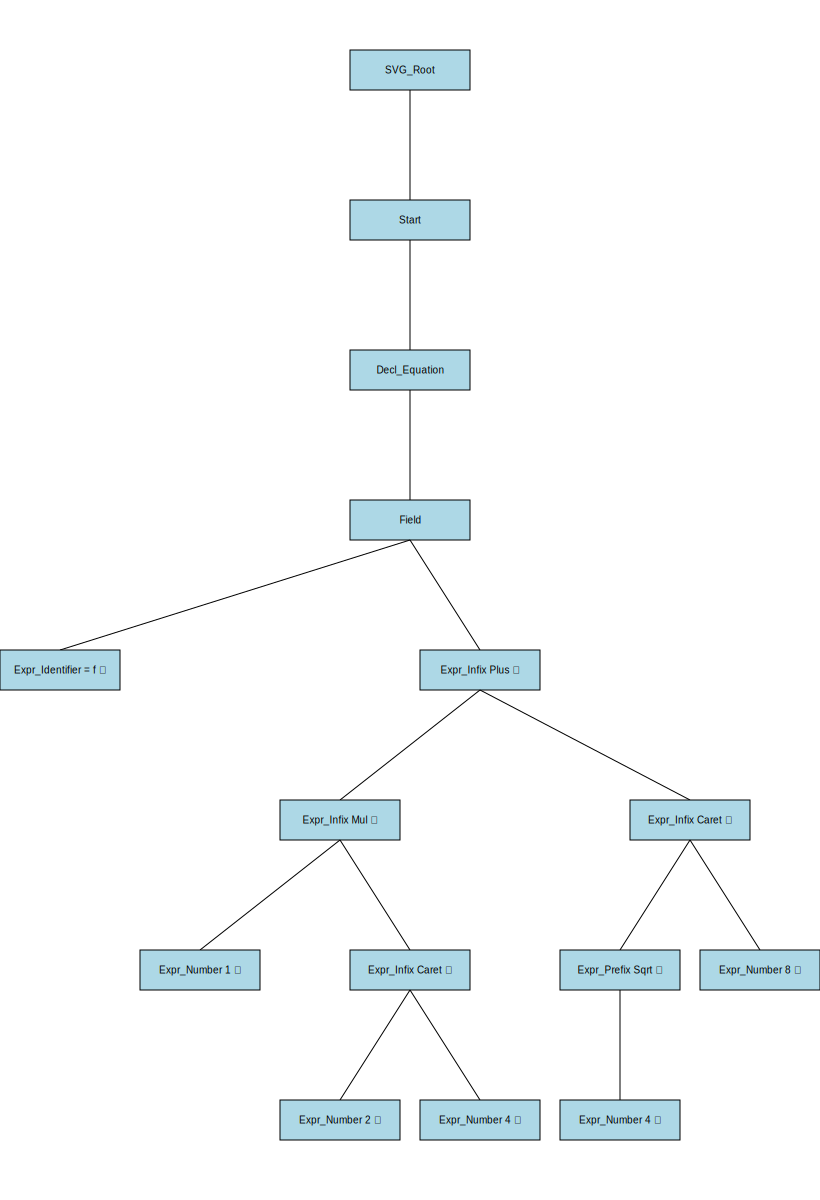
\includegraphics[width=\textwidth, scale=1.1]{./Imagens/svg.png}
        % 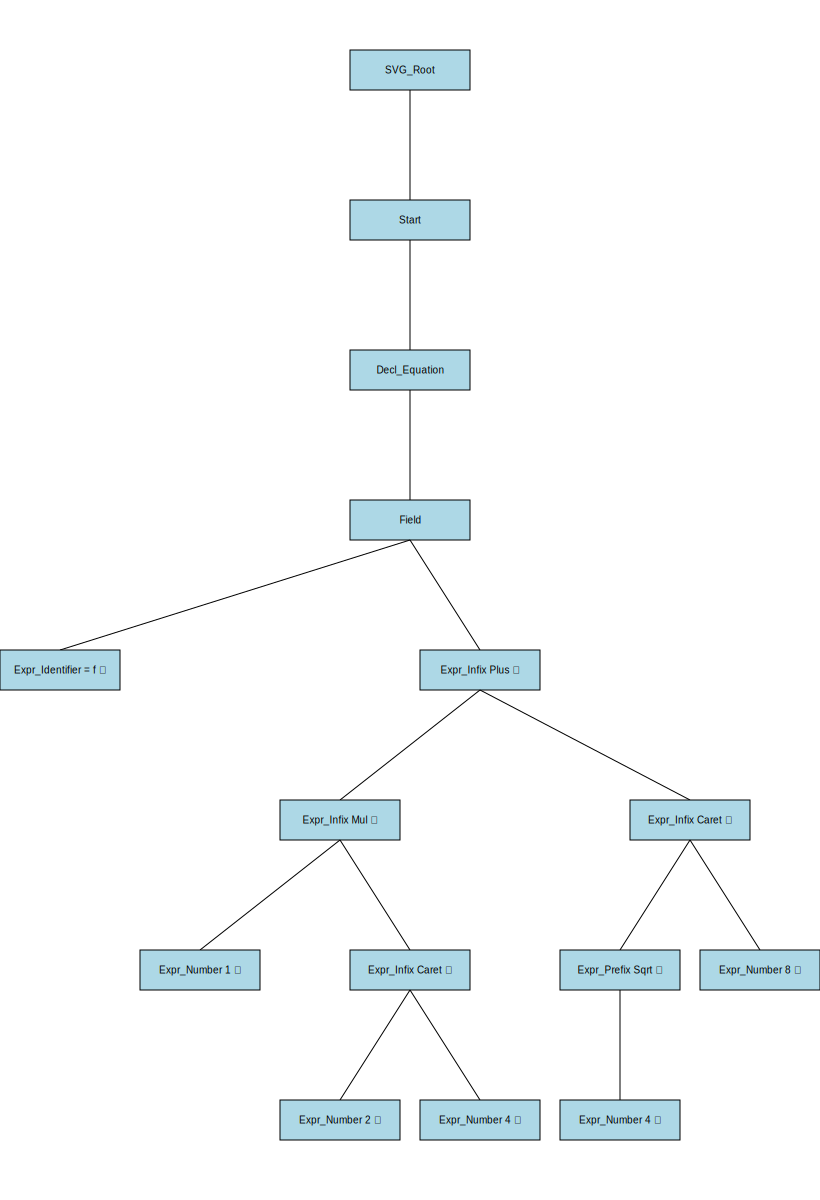
\includegraphics[scale=0.9]{./Imagens/svg.png}
        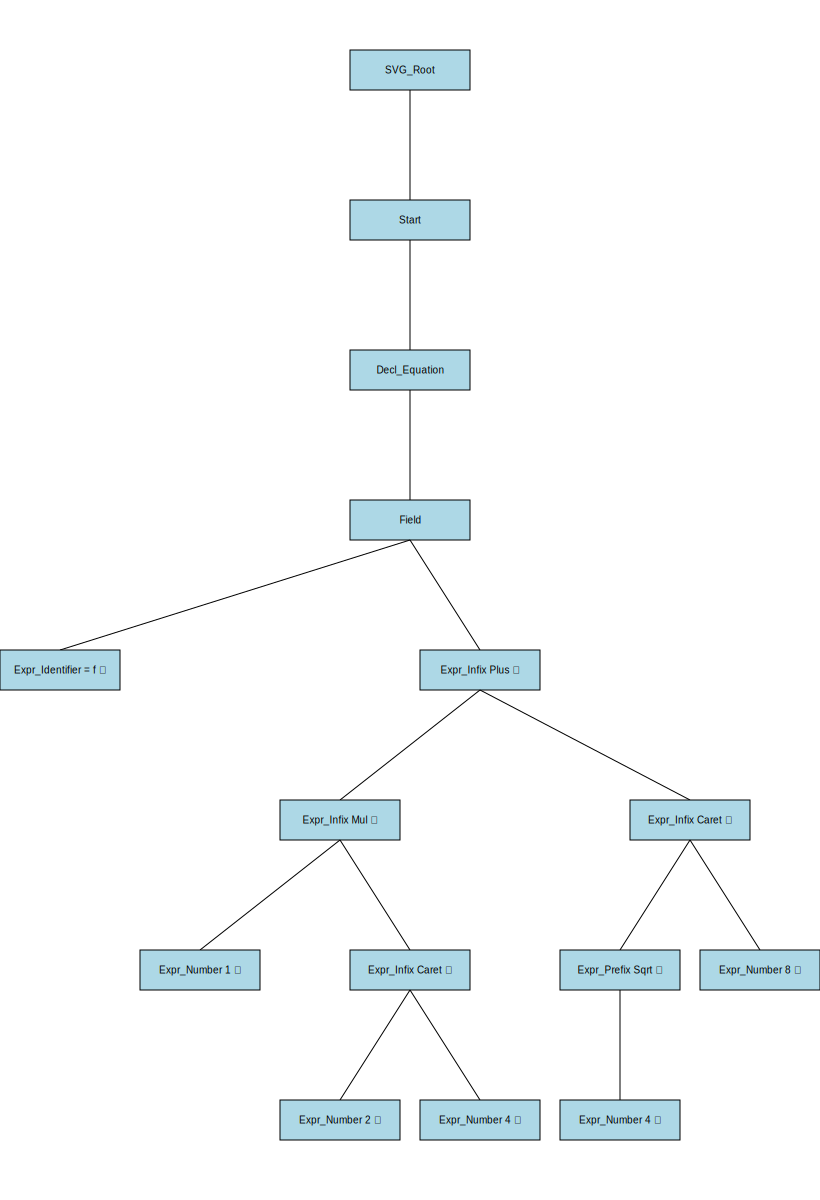
\includegraphics[scale=0.65]{./Imagens/svg.pdf} % Best outta of them all, because it gets to indefinitely zoom in
        % \includesvg[scale=0.9]{./Imagens/svg.svg}
    \end{center}
\end{figure}



% Temos dois tipos de validação dessa precendencia para garantir corretude de implementação de Pratt Parser, uma visual e outra automatica.
% Como mostrado em \autoref{tab-token-precedence} usamos uma tabela para definir a priopridade de operadores,
%
%
% ```
% \begin{equation}
% opertattions ungrouped
%
% \end{equation}
% ```
% Já se agruparmos certas operações, temos e o SVG gerado é diferente mostrando mostrando-se util em auxiliar o desenvolvimento.
%
%
% ```
% \begin{equation}
% grouped
% \end{equation}
% ```
% A maneira automatica é feita utilizando tested que gerandados sobre os casos, cada caso tem um entrada dada e saida esperada. A entrada é uma equação em string, a saída é uma string com a mesma, mas com a ordem de operação explicitamente citada através de parensentese. à Medida que o compialdor foi sendo desenvolvido mais teste foram adicionado para previnir quebra do código a medida que o projeto foi avançando. Alguns exemplos se encontram em @@@ e a informação gerada após aplicar o texto esta em @@@. Adicionamos o parentese através de um outro modulo chamado ``walker``, nele temos acesso à funções como ``children`` que dado um nó abstrato, ele resolve qual o tipo resolvido e cria um array de nós, como extrair os filho de nós heterogeneos precisa ser abstraido, cada estruttura tem campos diferetnes como filho. Outra facilidade que esse pacote desenvolvido é o padrão visitador @@ pegar o padrão visitador que tem função que utiliza generics.
%
%
% ```odin
% SVG_Node :: struct{
%     name: string,
%     children: [dynamic]^SVG_Node,
% };
% ```
% Como mostrado em @@@ usamos uma tabela para definir a priopridade de operadores
% Criamos um tabela que define e atráves de uma função, podemos acessar esses valores
% dado um token temos o reusltado
% Temos dois tipos de validação dessa precendencia para garantir correture de implementação de Pratt Parser, uma visual e outra automatica.
% Para validação visual, foi implementado um função que gera uma imagem no formato ``svg`` da arvore contendo informação circulos, representados nós da AST, jutamente com textos subinscritos informados metadados sobre os nós, como o tipo de operador, o tipo de nó, a string do indetificador  no caso de ser @etc
% Os nós próximo da raiz seriam implementados depois, já os proximos das folhas deve ser resolvikdos pprimeiros indicando um precedencia maior por exemplo
%
% Compilado para gerar a AST em SVG da equação @@, esperamos que '^' ocorra antes '*' que ocorra antes. Ao observar a arvore, notamos que o nó correspondente àoperação '^' ocorre.
%
% ```
% \begin{equation}
% opertattions ungrouped
%
% \end{equation}
% ```
% Já se agruparmos certas operações, temos e o SVG gerado é diferente mostrando mostrando-se util em auxiliar o desenvolvimento.
%
%
% ```
% \begin{equation}
% grouped
% \end{equation}
% ```
% A maneira automatica é feita utilizando tested que gerandados sobre os casos, cada caso tem um entrada dada e saida esperada. A entrada é uma equação em string, a saída é uma string com a mesma, mas com a ordem de operação explicitamente citada através de parensentese. à Medida que o compialdor foi sendo desenvolvido mais teste foram adicionado para previnir quebra do código a medida que o projeto foi avançando. Alguns exemplos se encontram em @@@ e a informação gerada após aplicar o texto esta em @@@. Adicionamos o parentese através de um outro modulo chamado ``walker``, nele temos acesso à funções como ``children`` que dado um nó abstrato, ele resolve qual o tipo resolvido e cria um array de nós, como extrair os filho de nós heterogeneos precisa ser abstraido, cada estruttura tem campos diferetnes como filho. Outra facilidade que esse pacote desenvolvido é o padrão visitador @@ pegar o padrão visitador que tem função que utiliza generics.
%
%
% ```odin
% SVG_Node :: struct{
%     name: string,
%     children: [dynamic]^SVG_Node,
% };
% ```
%
%
% \subsection{Testes}
%
%
% Foi desenvolvida uma série de testes que  abrangem vários aspectos da funcionalidade do \textit{parser}, incluindo geração de árvore de sintaxe, precedência de operadores e interpretação semântica.
%
%
% \subsubsection{Geração de Árvore de Sintaxe}
%
%
% Um aspecto crucial dos testes envolve verificar a correta geração de árvores sintáticas a partir de expressões de entrada. Os testes são projetados para cobrir diferentes cenários, incluindo operações aritméticas simples, expressões complexas com sub-expressões aninhadas e chamadas de funções. São eles:
%
%
% \begin{itemize}
%     \item O manuseio correto de operadores unários e binários, garantindo a precedência e associatividade adequadas.
%     \item A representação precisa de chamadas de função e seus argumentos dentro da árvore de sintaxe.
%     \item O agrupamento adequado de expressões dentro de parênteses para confirmar regras de precedência.
% \end{itemize}
